\chapter{System Design} \label{sec:SystemDesign}

The rapid urban forest assessment system requires a robust and scalable architecture capable of handling large-scale tree inventory data while providing real-time query capabilities for municipal planners and environmental researchers. Building upon the performance analysis presented in Chapter 3, which demonstrated that indexed database queries achieve 95\% performance improvements over non-indexed approaches, this chapter outlines the comprehensive system design that enables efficient processing and visualization of urban forest data across California's 702+ cities.

The system architecture addresses three critical design requirements: scalability to accommodate the 7.2 million tree records in the California Urban Forest Inventory, performance optimization to support interactive web applications with sub-second response times, and extensibility to incorporate additional environmental datasets and analysis capabilities. The design leverages cloud-native technologies and modern web frameworks to create a maintainable and cost-effective solution.

\section{System Diagram}
\label{subsec:diagram}

\begin{figure}[H]
\centering
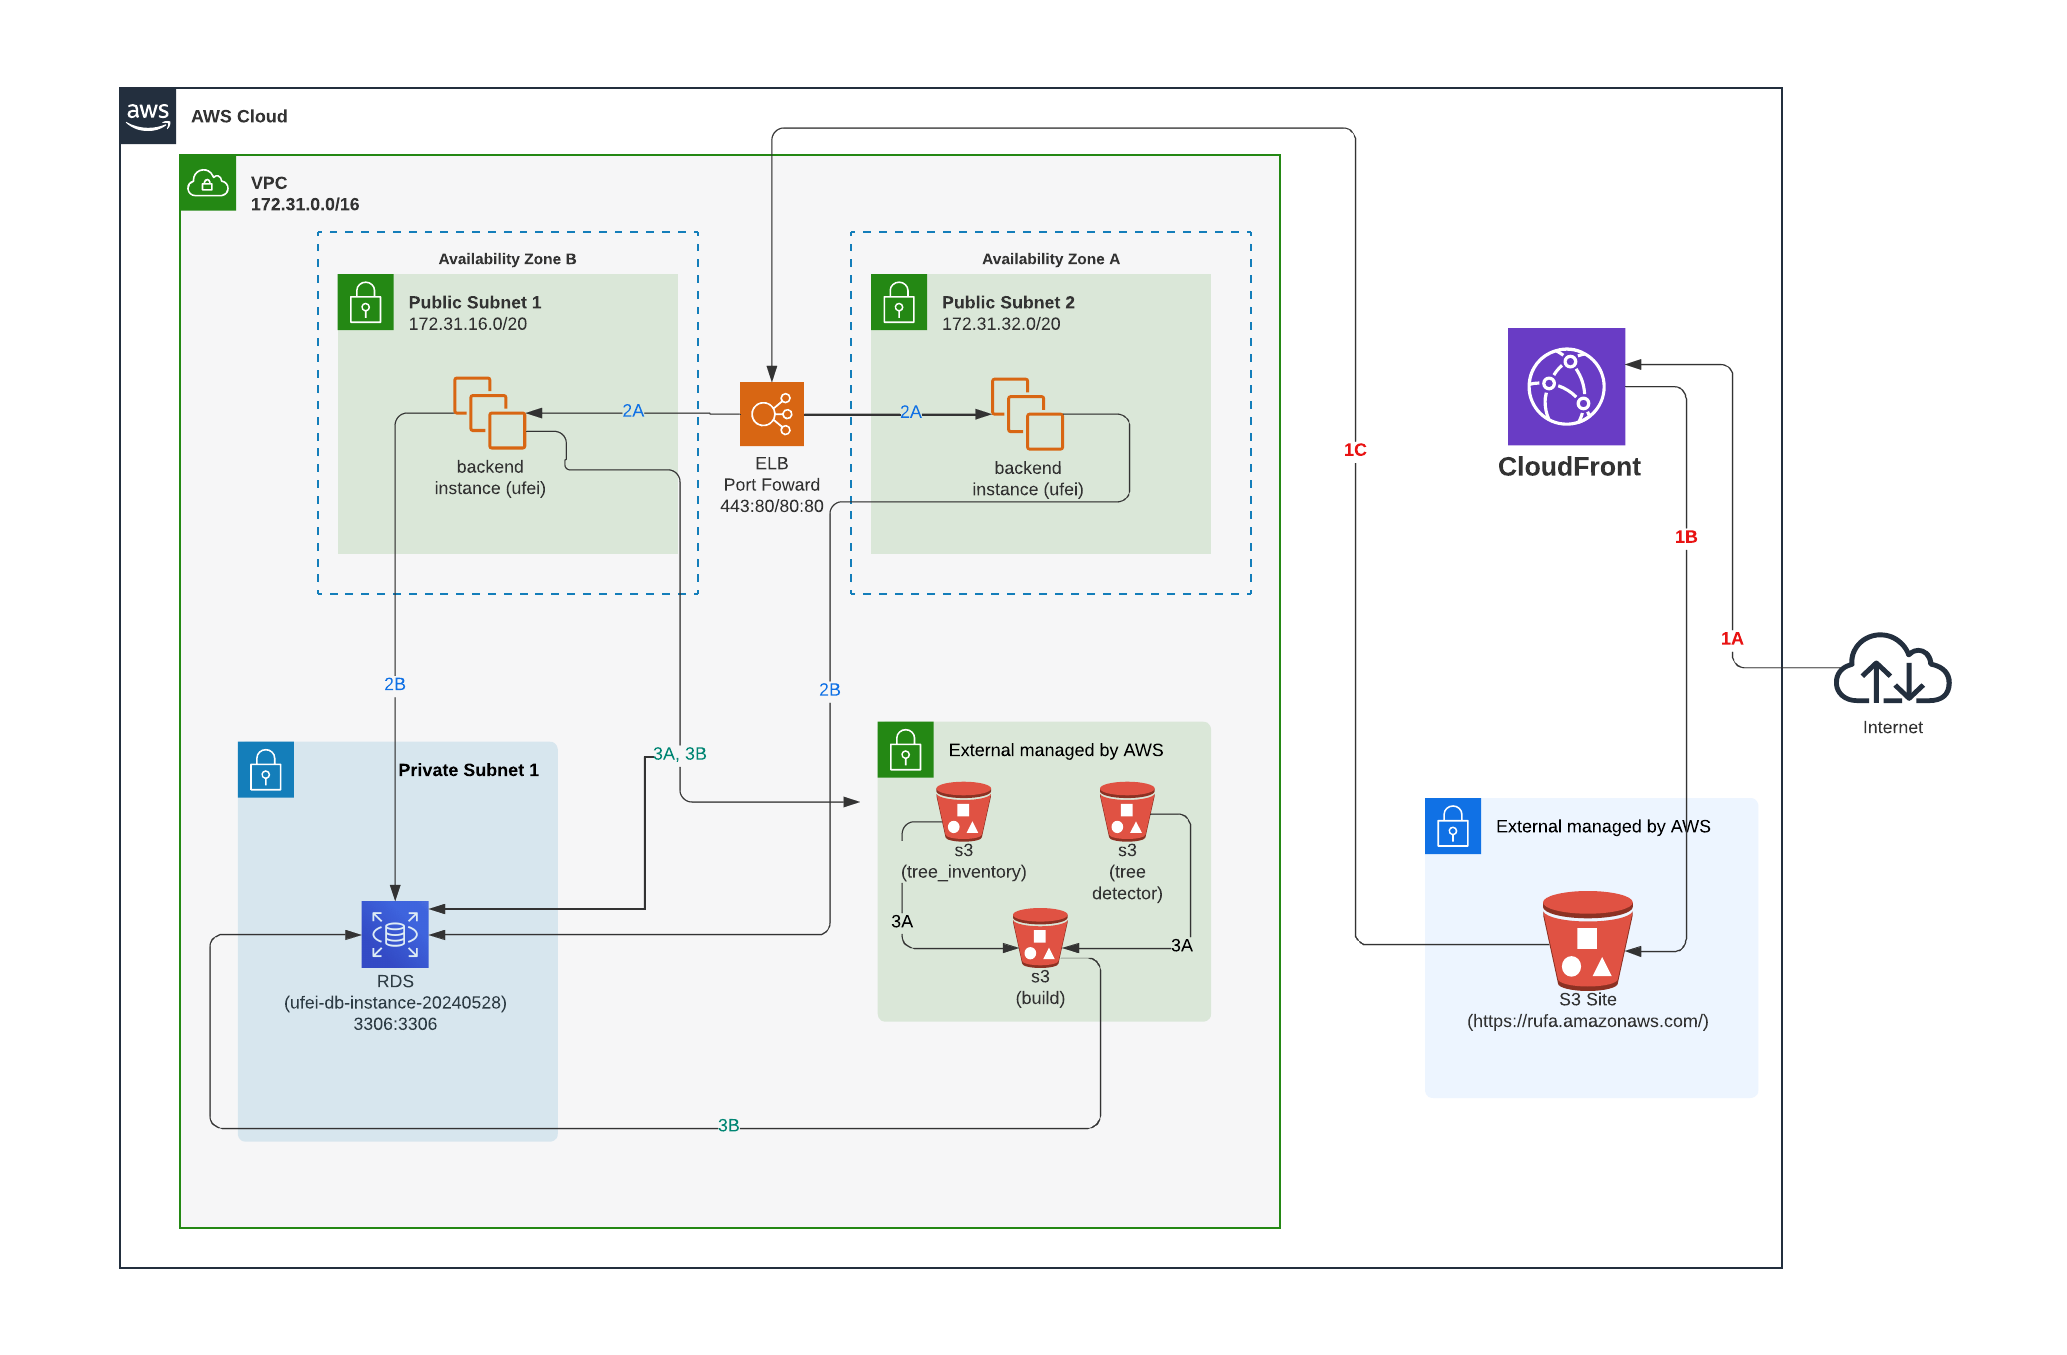
\includegraphics[width=0.95\textwidth]{figures/rufa_system.png}
\caption{AWS-based system architecture for the RUFA platform.}
\label{fig:rufa_system_architecture}
\end{figure}

Figure~\ref{fig:rufa_system_architecture} presents the architecture of the RUFA system, deployed within an AWS Virtual Private Cloud (VPC) for scalability, security, and high availability. The system follows a three-tier design: front-end delivery, backend processing, and data storage.

\begin{table}[h!]
\centering
\caption{System Component Connections}
\label{tab:system_connections}
\begin{tabular}{p{2cm}p{3cm}p{6cm}}
\hline
\textbf{Connection} & \textbf{From} & \textbf{To} \\
\hline
1A & Users & CloudFront CDN \\
1B & CloudFront & S3 Static Assets \\
1C & CloudFront & Backend Services \\
2A & ELB & EC2 Instances \\
2B & ELB & HTTPS/HTTP Requests \\
3A & Backend & RDS MySQL Database \\
3B & Backend & S3 Data Buckets \\
\hline
\end{tabular}
\end{table}

Users access the dashboard through CloudFront (1A), which delivers static web assets hosted on Amazon S3 (1B) and routes data requests (1C) to backend services inside the VPC. Backend processing occurs on EC2 instances (2A) distributed across two availability zones, managed by an Elastic Load Balancer (ELB) that forwards HTTPS and HTTP requests (2B). These instances handle user queries, filtering, and aggregation tasks such as computing city-level tree density or generating spatial histograms.

The data layer includes an Amazon RDS MySQL database in a private subnet, securely accessed only by backend instances. Supporting geospatial and inventory datasets are stored in S3 buckets (3A, 3B), which hold tree inventory, canopy detection, and build artifacts. This configuration enables distributed computation on subsets of data for each city or ZIP code.

This architecture enables rapid querying, scalable data processing, and real-time visualization of over seven million urban tree records across California's cities, providing urban planners and environmental researchers with the tools necessary for sustainable planning and evidence-based decision-making.

